\documentclass[tikz,border=3mm,multi=tikzpicture]{standalone}
\usepackage[utf8]{inputenc}
\usepackage[T1]{fontenc}
\usepackage{helvet}
\renewcommand{\familydefault}{\sfdefault}
\usepackage{tikz}
\usetikzlibrary{angles,quotes,calc,intersections}
\begin{document}

\tikzset{every node/.append style={font=\sffamily\small}}
% TikZ 1
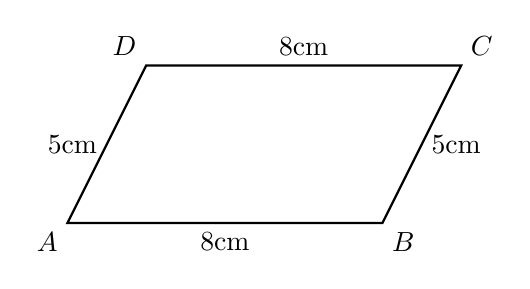
\begin{tikzpicture}[scale=1]
\coordinate (A) at (0,0); \coordinate (B) at (4,0); \coordinate (C) at (5,2); \coordinate (D) at (1,2);
\draw[thick] (A)--(B)--(C)--(D)--cycle;
\node[below] at ($(A)!0.5!(B)$) {$8\mathrm{cm}$};
\node[above] at ($(D)!0.5!(C)$) {$8\mathrm{cm}$};
\node[left] at ($(A)!0.5!(D)$) {$5\mathrm{cm}$};
\node[right] at ($(B)!0.5!(C)$) {$5\mathrm{cm}$};
\foreach \p/\pos in {A/below left,B/below right,C/above right,D/above left}{\node[\pos] at (\p) {$\p$};}
\end{tikzpicture}
% TikZ 2
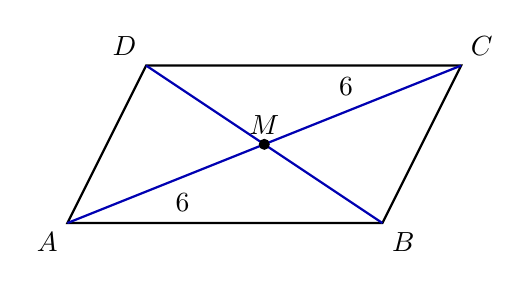
\begin{tikzpicture}[scale=1]
\coordinate (A) at (0,0); \coordinate (B) at (4,0); \coordinate (C) at (5,2); \coordinate (D) at (1,2);
\coordinate (M) at ($(A)!0.5!(C)$);
\draw[thick] (A)--(B)--(C)--(D)--cycle;
\draw[blue!70!black,thick] (A)--(C);
\draw[blue!70!black,thick] (B)--(D);
\fill (M) circle (2pt);
\node[above] at (M) {$M$};
\node[below right] at ($(A)!0.5!(M)$) {$6$};
\node[above left] at ($(M)!0.5!(C)$) {$6$};
\foreach \p/\pos in {A/below left,B/below right,C/above right,D/above left}{\node[\pos] at (\p) {$\p$};}
\end{tikzpicture}


% TikZ 3
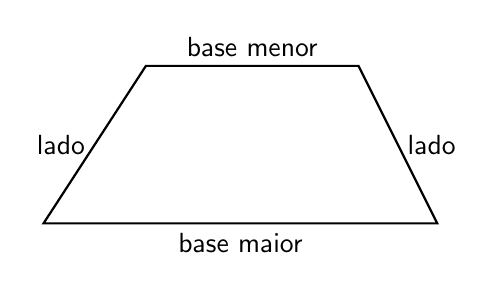
\begin{tikzpicture}[scale=1]
\coordinate (A) at (0,0); \coordinate (B) at (5,0); \coordinate (C) at (4,2); \coordinate (D) at (1.3,2);
\draw[thick] (A)--(B)--(C)--(D)--cycle;
\node[below] at ($(A)!0.5!(B)$) {base maior};
\node[above] at ($(D)!0.5!(C)$) {base menor};
\node[left] at ($(A)!0.5!(D)$) {lado};
\node[right] at ($(B)!0.5!(C)$) {lado};
\end{tikzpicture}
% TikZ 4
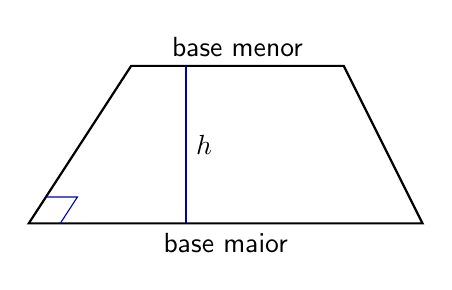
\begin{tikzpicture}[scale=1]
\coordinate (A) at (0,0); \coordinate (B) at (5,0); \coordinate (C) at (4,2); \coordinate (D) at (1.3,2);
\draw[thick] (A)--(B)--(C)--(D)--cycle;
\draw[blue!70!black,thick] (2,0)--(2,2);
\pic[draw=blue!70!black, angle radius=4mm] {right angle=B--A--D};
\node[right] at (2,1) {$h$};
\node[below] at (2.5,0) {base maior};
\node[above] at (2.65,2) {base menor};
\end{tikzpicture}
\end{document}
